\documentclass{article}
\usepackage[margin = 2.54cm]{geometry} % set margin to traditional doc

%packages
\usepackage{graphicx} % Required for inserting images
\usepackage[most]{tcolorbox} %for creating environments
\usepackage{amsmath}
\usepackage{amssymb}
\usepackage{verbatim}
\usepackage[utf8]{inputenc}
\usepackage[dvipsnames]{xcolor} %for importing multiple colors
\usepackage{hyperref} %for creating links to different sections
\usepackage{tikz} %for certain graph drawing

\linespread{1.2} %controlling line spread

%define colors i like
\definecolor{myTeal}{RGB}{0,128,128}
\definecolor{myGreen}{RGB}{34,170,34}
\definecolor{mySapphire}{RGB}{15,82,186}
\definecolor{myEmerald}{RGB}{50.4, 130, 90}

%create math environments, can add [section] or [subsection] to add index counter based on sections/subsections
\newtheorem{define}{Definition}
\newtheorem{prop}{Proposition}
\newtheorem{thm}{Theorem}
\newtheorem{question}{Question}
\newtheorem{lemma}{Lemma}
\newtheorem{code}{Code}

%setup colored box environment for each math env above
\tcolorboxenvironment{define}{
    enhanced, colframe=myTeal!50!teal, colback=myTeal!10,
    arc=5mm, lower separated=false, fonttitle=\bfseries
}
\tcolorboxenvironment{prop}{
    enhanced, colframe=myGreen!50!black, colback=myGreen!15,
    arc=5mm, lower separated=false, fonttitle=\bfseries
}
\tcolorboxenvironment{thm}{
    enhanced, colframe=mySapphire!50!mySapphire, colback=mySapphire!15,
    arc=5mm, lower separated=false, fonttitle=\bfseries
}
\tcolorboxenvironment{question}{
    enhanced, colframe=blue!50!black, colback=blue!10,
    arc=5mm, lower separated=false, fonttitle=\bfseries
}
\tcolorboxenvironment{lemma}{
    enhanced, colframe=myEmerald!50!myEmerald, colback=myEmerald!10,
    arc=5mm, lower separated=false, fonttitle=\bfseries
}
\tcolorboxenvironment{code}{
    enhanced, colframe=myEmerald!50!myEmerald, colback=myEmerald!10,
    arc=5mm, lower separated=false, fonttitle=\bfseries
}

%setup hyperlink within pdf
\hypersetup{
    colorlinks=true,
    linkcolor=blue,
    filecolor=magenta,      
    urlcolor=cyan,
    pdftitle={Overleaf Example},
    pdfpagemode=FullScreen,
}

%common command (add to template)
%general
\newcommand{\FF}{\mathbb{F}}
\newcommand{\NN}{\mathbb{N}}
\newcommand{\ZZ}{\mathbb{Z}}
\newcommand{\QQ}{\mathbb{Q}}
\newcommand{\RR}{\mathbb{R}}
\newcommand{\CC}{\mathbb{C}}

\newcommand{\Id}{\textmd{Id}} %identity
\newcommand{\lcm}{\textmd{lcm}}

%algebra
\newcommand{\Gal}{\textmd{Gal}}
\newcommand{\Aut}{\textmd{Aut}}
\newcommand{\End}{\textmd{End}}
\newcommand{\Coker}{\textmd{Coker}}
\newcommand{\Hom}{\textmd{Hom}}

%analysis
\newcommand{\Vol}{\textmd{Vol}}

%complex
\newcommand{\Real}{\textmd{Re}}
\newcommand{\Imag}{\textmd{Im}} %can also be used for Image
\newcommand{\Res}{\textmd{Res}}

%lie algebra
\newcommand{\gl}{\mathfrak{gl}}

%physics
\newcommand{\br}{\overline{r}}
\newcommand{\bv}{\overline{v}}
\newcommand{\ba}{\overline{a}}
\newcommand{\bzero}{\overline{0}}
\newcommand{\bF}{\overline{F}}

\title{Phys 103 HW1}
\author{Zih-Yu Hsieh}

\begin{document}
\maketitle

\section{}%1
\begin{question}\label{q1}
    Consider a puck sliding across a frictionless merry-go-round at speed $v$ on a trajectory which passes through the center. The merry-go-round rotates at angular velocity $w$ and has radius $R$.
    \begin{itemize}
        \item[(a)] Write down the $r,\phi$ coordinates of the puck as functions of time, as observed by an observer standing next to the merry-go-round. Take $t=0$ to be the time when the puck is at the edge of the merry-go-round, the spatial origin to be at the center of the merry-go-round, and $\phi=0$ to be the initial angular location of the puck. Is the observer in an inertial frame?
        \item[(b)] Write down the $r', \phi'$ coordinates of the puck as functions of time, as observed by an observer sitting on the edge of the merry-go-round. Take $t=0$ to be the time when the puck is at the edge of the merry-go-round, the spatial origin to be at the center of the merry-go-round, and $\phi'=0$ to be the initial angular location of the puck. Is the observer in an inertial frame?
    \end{itemize}
\end{question}

\textbf{Pf:}

For both parts, we'll assume that the codomain of $r,\phi$ is $\RR$ (i.e. allows negative radius $r$ for simplicity).
\subsection*{(a)}
First, we'll consider the distance of the puck away from the origin: On the $1$-dimensional trajectory, assume the origin (center) is position $r=0$, and at $t=0$, the puck is at the edge, which has position $r=R$ (assume that the puck initially has positive value position in the coordinate, so the distance from the center to the edge is the radius). Assume the puck is traveling in radial direction, relative to
 the track its velocity is given by $v$, hence the position $r(t) = \int vdt = vt+C$. With $r(0) = 0+C = R$, we have $r(t)=R+vt$. This records the radial distance of the puck from the origin.

Now, we'll consider the angle of the puck relative to the observer (which we'll keep track of the angle of its initial position on the trajectory, since no matter where the puck is on the trajectory, because the trajectory passes through the center, the puck's angle is the same as the trajectory): With initial angle $\phi(0) = 0$, and angular velocity $w$, then the angle $\phi(t) = \int w dt = wt + C$. Where with $\phi(0) = 0+C = 0$, we have $\phi(t) = wt$.

\hfil

With $(r,\phi)$ being the given polar coordinates of the puck, in cartesian coordinates, the position is given by:
$$\br(t)=(r\cos(\phi),r\sin(\phi)) = (R+vt)(\cos(wt),\sin(wt))$$
Taking derivative, we get the velocity as follow:
$$\bv(t) = (v\cos(wt)-w(R+vt)\sin(wt), v\sin(wt)+w(R+vt)\cos(wt))$$
Taking the second derivative, we get the acceleration as follow:
$$\ba(t) = (-wv\sin(wt)- w(v\sin(wt) + w(R+vt)\cos(wt)), wv\cos(wt) + w(v\cos(wt)-w(R+vt)\sin(wt)))$$
$$ = (-2wv\sin(wt) - w^2(R+vt)\cos(wt), 2wv\cos(wt)-w^2(R+vt)\sin(wt))$$
Which, plug in $t=0$, we get $\ba(0) = (-w^2R, 2wv) \neq \bar{0}$, showing that there are time where the puck is under acceleration. If we assume the puck is an isolated object, then because for the observer the puck is accelerating, the observer is not in an inertial frame.

\subsection*{(b)}
When considering the distance of the puck away from the origin, using similar coordinates from part (a), assume the center has radius $r=0$, the puck initially has radius $r=R$, and the puck has speed $v$ in radial direction, then the position of the puck is again given as $r(t)=R+vt$ (the same derivation).

In contrast, for the angle $\phi$, since the observer is now on the edge of the merry-go-round, then the relative angle in between the observer and the puck's initial position never changes. So, $\phi(t)=0$ (where the initial angle of the puck is).

\hfil

With $(r,\phi)$ given as the polwer coordinates of the puck, in cartesian coordinates, the position is given by:
$$\br(t) = (r\cos(\phi), r\sin(\phi)) = (R+vt)(1,0) = (R+vt,0)$$
Hence, taken second derivative, we get the acceleration as follow:
$$\ba(t) = \bzero$$
If treating the puck as an isolated object again, then this observer is in an inertial frame (since the isolated object is not accelerating).

\break

\section{}%2
\begin{question}\label{q2}
    Consider an athlete putting a shot. Naturally, she would like to maximize the distance the shot travels. If the shot is put from a height $h$ and with initial speed $v_0$, what launch angle maximizes the distance traveled? Assume that $v_0$ and $h$ are independent of the launch angle, and ignore air resistance (but include gravity, if it wasn't obvious). You can (and should) assume that $h$ is "small" and give an answer to leading non-trivial order, but you should specify what counts as "small".
\end{question}

\textbf{Pf:}

We'll assume the vertical direction upward is the $\hat{y}$ axis, while the horizontal direction (where the shot is heading horizontally) is the $\hat{x}$ axis. We'll also assume the initial position of the shot $\br(0) = (0,h)$, and let $\theta$ represents the initial launching angle.

Since the only force taking into account is gravity, then the net force acting on the launch is $\bF_{net} = \bF_g = -mg\hat{y}$, hence the acceleration is given by $\ba = \frac{1}{m}\bF_{net} = -g\hat{y}$ (here assumes the mass of the shot is constant).

Taking integration, we get $\bv(t) = \int \ba dt = -gt\hat{y}+\overline{C}$ for some $\overline{C} \in \RR^2$. Which, recall that initial velocity has speed $v_0$ and launch angle $\theta$, hence $\bv(0) = (v_0\cos(\theta),v_0\sin(\theta)) = 0\cdot \hat{y}+\overline{C}$. Which, $\bv(t) = (v_0\cos(\theta), v_0\sin(\theta)-gt)$.

Then, taking integration again, we get $\br(t) = \int \bv dt = (v_0\cos(\theta)t + r_x, v_0\sin(\theta)t - \frac{1}{2}gt^2 + r_y)$ for some $(r_x,r_y)\in \RR^2$, and with the assumption that $\br(0) = (0,h) = (0+r_x, 0-0+r_y)$, we get the following for position:
$$\br(t) = \left(v_0\cos(\theta)t, v_0\sin(\theta)t-\frac{1}{2}gt^2+h\right)$$

\hfil

Now, the objective is to solve for the horizontal distance the shot would travel, which we need to calculate the time it lands (i.e. the second coordinate of $\br(t)$ is 0). For $-\frac{1}{2}gt^2+v_0\sin(\theta)t+h = 0$, using quadratic formula, we get the following expression for $t$:
$$t = \frac{-v_0\sin(\theta)\pm \sqrt{v_0^2\sin^2(\theta)-4\cdot \left(-\frac{g}{2}\right)h}}{2\left(-\frac{g}{2}\right)} = \frac{v_0\sin(\theta)\pm\sqrt{v_0^2\sin^2(\theta)+2gh}}{g}$$
Since we can assume both $g,h>0$ (it's not reasonable to launch a shot from height $h<0$ in general), hence $(v_0^2\sin^2(\theta)+2gh)\geq v_0^2\sin^2(\theta)$, showing that $\sqrt{v_0^2\sin^2(\theta)+2gh} \geq |v_0\sin(\theta)|\geq v_0\sin(\theta)$. So, for $t>0$, we need positive sign for the square root, getting that the landing time is as follow:
$$t=\frac{v_0\sin(\theta)+\sqrt{v_0^2\sin^2(\theta)+2gh}}{g}$$
Since the launch starts at time $=0$, then the above time is exactly the time where the shot is in the air. Hence, the horizontal distance traveled is given by:
$$\Delta x=v_0\cos(\theta)t = v_0\cos(\theta)\cdot\frac{v_0\sin(\theta)+\sqrt{v_0^2\sin^2(\theta)+2gh}}{g} = v_0^2\sin(\theta)\cos(\theta)\frac{1+\sqrt{1+\frac{2gh}{v_0^2\sin^2(\theta)}}}{g}$$
This expression is relatively hard to solve for the maximum value with $\theta$, so using Taylor polynomial to approximate for the square root term is necessary.

Assume $\theta\in [k,\frac{\pi}{2}]$ for some $k>0$, or else the $\sin(\theta)$ in the denominator could go unbounded, if assume $h$ is small, can also assume $\frac{2gh}{v_0^2\sin^2(\theta)}$ is small, then the taylor polynomial of $\sqrt{1+x}$ could yield a good approximation (also, since for $h=0$, optimal angle $\theta=\frac{\pi}{4}$, physically it's also good to assume the angle is close to $\frac{\pi}{4}$, hence the input term is bounded). For $x$ close to $0$, up to linear order, its taylor polynomial is given as follow:
$$\sqrt{1+x}\approx 1+\frac{1}{2}x$$
Using this approximation for $x=\frac{2gh}{v_0^2\sin^2(\theta)}$, the horizontal displacement is approximated as follow:
$$\Delta x\approx v_0^2\sin(\theta)\cos(\theta)\cdot\frac{1+\left(1+\frac{1}{2}\cdot\frac{2gh}{v_0^2\sin^2(\theta)}\right)}{g} = \frac{2v_0^2}{g}\sin(\theta)\cos(\theta)+h\cdot\frac{\cos(\theta)}{\sin(\theta)} = \frac{2v_0^2}{g}\sin(\theta)\cos(\theta)+h\cot(\theta)$$
To get a local maximum, differentiate the above term with respect to $\theta$, we get:
$$\frac{d}{d\theta}\Delta x=\frac{2v_0^2}{g}(\cos^2(\theta)-\sin^2(\theta))-h\csc^2(\theta)=\frac{2v_0^2}{g}(1-2\sin^2(\theta))-\frac{h}{\sin^2(\theta)}$$
With the above expression being $0$, we get:
$$\frac{2v_0^2}{g}(1-2\sin^2(\theta))-\frac{h}{\sin^2(\theta)}=0 \implies (2\sin^2(\theta)-1)\sin^2(\theta)+\frac{gh}{2v_0^2}=0$$
With $x:=\sin^2(\theta)$, we get:
$$2x^2-x+\frac{gh}{2v_0^2}=0 \implies x=\sin^2(\theta)=\frac{1\pm\sqrt{1-\frac{4gh}{v_0^2}}}{4}$$
With the assumption that $\theta \geq k>0$, and $h$ being extremely small, then $\sqrt{1-\frac{4gh}{v_0^2}}$ would be pretty close to $1$, hence the negative sign would provide that $\sin^2(\theta)$ is approximately $0$, so we'll take the positive sign.

Finally, this indicates the angle $\theta$ for maximum launch distance is approximated as follow:
$$\sin^2(\theta)=\frac{1}{4}\left(1+\sqrt{1-\frac{4gh}{v_0^2}}\right)\implies \sin(\theta)=\frac{1}{2}\sqrt{1+\sqrt{1-\frac{4gh}{v_0^2}}}$$
$$\implies \theta = \arcsin\left(\frac{1}{2}\sqrt{1+\sqrt{1-\frac{4gh}{v_0^2}}}\right)$$

\break

\begin{comment}
\section{}%3
\begin{question}\label{q3}
    Consider an object, such as a car, with mass $m$, starting from rest, moving in one dimension, and subject to two forces. One, provided by an engine with a certain power output, is $F_e = P/v$. The other is some quadratic drag from air resistance, $F_d = -cv^2$.$P,c$ are both positive constants. Unfortunately, it is not possible to analytically solve for the car's velocity as a function of time. However, we can get approximate analytic expressions which are very accurate.
    \begin{itemize}
        \item[(a)] First, nondimensionalize your equation, defining appropriate dimensionless time and velocity variables.
        \item[(b)] At the start of the motion, $\tilde{v}<< 1$, so air resistance is a small correction; the car's motion is essentially just acceleration driven by the engine. By ignoring the force due to air resistance, determine an (approximate) formula $\tilde{v}(\tilde{t})$, valid for $\tilde{v}<<1$.
        \item[(c)]Eventually, the car approaches terminal velocity. We can define 
        $$\epsilon = \tilde{v}_t-\tilde{v}$$
        If the car is going close to terminal velocity, $\epsilon <<1$. Expand the forces to linear order in $\epsilon$, and solve to get an (approximate) formula $\epsilon(\tilde{t})$, valid for $\epsilon<<1$.
        \item[(d)] Now comes the leap of faith: assume that either the velocity is small enough to ignore air resistance or the velocity is close to terminal velocity. In other words, we'll write $\tilde{v}(\tilde{t})$ as a piecewise function; before some time $\tilde{t}_*$ it takes the form of your solution to (c). Choose an appropriate switching time $\tilde{t}_*$ and write down such a piecewise function for $\tilde{v}(\tilde{t})$. You should fix the two undetermined constants by using that (i) the car starts at rest and (ii) $\tilde{v}$ should be continuous.Plot the piecewise function $\tilde{v}(\tilde{t})$.
        \item[(e)] Put all the constants back in to get $v(t)$. At what time $t$ does the car obtain $99\%$ of terminal velocity? You should give an analytic expression (using your approximate $\tilde{v}$). 
    \end{itemize}
\end{question}

\textbf{Pf:}
\subsection*{(a)}
Given that force $F=m\frac{dv}{dt}=F_e + F_d$, we get the following differential equation:
$$m\frac{dv}{dt}=\frac{P}{v}-cv^2$$
For some non-determined constant velocity $v_0$ and time $t_0$, let $\tilde{v}=\frac{v}{v_0}$, $\tilde{t}=\frac{t}{t_0}$, then we get the following expression:
$$\frac{d\tilde{v}}{d\tilde{t}} = \frac{d}{d\tilde{t}}\left(\frac{v(t)}{v_0}\right) = \frac{1}{v_0}\cdot \frac{dv}{dt}\cdot \frac{dt}{d \tilde{t}} = \frac{t_0}{v_0}\frac{dv}{dt}$$
Substituting all the expressions of $v$ and $t$, we get:
$$m\cdot \frac{v_0}{t_0}\frac{d\tilde{v}}{d\tilde{t}} = \frac{P}{v_0\tilde{v}}-c(v_0\tilde{v})^2\implies \frac{d\tilde{v}}{d\tilde{t}}=\frac{t_0\cdot P}{mv_0^2}\cdot\frac{1}{\tilde{v}}-\frac{ct_0\cdot v_0}{m}\tilde{v}^2$$
If set $t_0=m$, and $v_0 = \sqrt{P}$, the above differential equation can be simplified as:
$$\frac{d\tilde{v}}{d\tilde{t}}=\frac{mP}{m(\sqrt{P})^2}\cdot\frac{1}{\tilde{v}}-\frac{cm\sqrt{P}}{m}\tilde{v}^2 = \frac{1}{\tilde{v}}-c\sqrt{P}\tilde{v}^2$$
This will be the nondimensionalized differential equation we use.

\hfil

\subsection*{(b)}
For $\tilde{v}<<1$, if we can assume air resistance is negligible, then $c=0$, hence the differential equation becomes:
$$\frac{d\tilde{v}}{d\tilde{t}}=\frac{1}{\tilde{v}} \implies \tilde{v}\frac{d\tilde{v}}{d\tilde{t}}=1\implies \int \tilde{v}\frac{d\tilde{v}}{d\tilde{t}}d\tilde{t} = \frac{1}{2}\tilde{v}^2 = \int 1d\tilde{t}=\tilde{t}+C$$
$$\implies \tilde{v}^2 = 2\tilde{t}+C' \implies \tilde{v}=\pm\sqrt{2\tilde{t}+C'}$$
With $\tilde{v}\geq 0$ (can assume it is traveling in the same direction), the positive sign can be chosen; and, since at $\tilde{t}=0$ (implying $t=0$), we have $\tilde{v}(0)=0$ (initially at rest), hence $\tilde{v}(0) = \sqrt{0+C'} = 0$, showing that $C' = 0$, or $\tilde{v}(\tilde{t}) = \sqrt{2\tilde{t}}$.

\hfil

\subsection*{(c)}
If define $\epsilon=\tilde{v_t}-\tilde{v}$ (with $\tilde{v_t}$ being a constant), then $\frac{d\epsilon}{d\tilde{t}} = - \frac{d\tilde{v}}{d\tilde{t}}$, and $\tilde{v}=\tilde{v_t}-\epsilon$. Then, the original differential equation becomes:
$$\frac{d\tilde{v}}{d\tilde{t}}=\frac{1}{\tilde{v}}-c\sqrt{P}\tilde{v}^2 \implies -\frac{d\epsilon}{d\tilde{t}} = \frac{1}{\tilde{v_t}-\epsilon}-c\sqrt{P}(\tilde{v_t}-\epsilon)^2 = \frac{1}{\tilde{v_t}}\cdot \frac{1}{1-\frac{\epsilon}{\tilde{v_t}}}-c\sqrt{P}(\tilde{v_t}-\epsilon)^2$$
If assume $\epsilon<<1$, can assume $|\frac{\epsilon}{\tilde{v_t}}|<1$, hence the taylor series of $\frac{1}{1-x}$ is given by $\sum_{n=0}^{\infty}x^n$. Taking up to linear term (for both the rational and the second degree polynomial), we get the following:
$$-\frac{d\epsilon}{d\tilde{t}}\approx \frac{1}{\tilde{v_t}}\left(1+\frac{\epsilon}{\tilde{v_t}}\right)-c\sqrt{P}(\tilde{v_t}^2-2\tilde{v_t}\epsilon) = \left(\frac{1}{\tilde{v_t}}-c\sqrt{P}\tilde{v_t}^2\right)+\left(\frac{1}{\tilde{v_t}^2}+2c\sqrt{P}\tilde{v_t}\right)\epsilon$$
$$\implies \frac{1}{\left(\frac{1}{\tilde{v_t}}-c\sqrt{P}\tilde{v_t}^2\right)+\left(\frac{1}{\tilde{v_t}^2}+2c\sqrt{P}\tilde{v_t}\right)\epsilon}\frac{d\epsilon}{d\tilde{t}} = -1$$
Taking integral on both sides with respect to $\tilde{t}$, we get:
$$\frac{1}{\left(\frac{1}{\tilde{v_t}^2}+2c\sqrt{P}\tilde{v_t}\right)}\ln\left(\left(\frac{1}{\tilde{v_t}}-c\sqrt{P}\tilde{v_t}^2\right)+\left(\frac{1}{\tilde{v_t}^2}+2c\sqrt{P}\tilde{v_t}\right)\epsilon\right) = -\tilde{t}+C$$
$$\implies\ln\left(\left(\frac{1}{\tilde{v_t}}-c\sqrt{P}\tilde{v_t}^2\right)+\left(\frac{1}{\tilde{v_t}^2}+2c\sqrt{P}\tilde{v_t}\right)\epsilon\right)=-\left(\frac{1}{\tilde{v_t}^2}+2c\sqrt{P}\tilde{v_t}\right)\tilde{t}+C'$$
$$\implies \left(\frac{1}{\tilde{v_t}}-c\sqrt{P}\tilde{v_t}^2\right)+\left(\frac{1}{\tilde{v_t}^2}+2c\sqrt{P}\tilde{v_t}\right)\epsilon = C''\exp\left(-\left(\frac{1}{\tilde{v_t}^2}+2c\sqrt{P}\tilde{v_t}\right)\tilde{t}\right)$$
$$\implies \epsilon = C'''\exp\left(-\left(\frac{1}{\tilde{v_t}^2}+2c\sqrt{P}\tilde{v_t}\right)\tilde{t}\right)-\left(\frac{1}{\tilde{v_t}}-c\sqrt{P}\tilde{v_t}^2\right)/\left(\frac{1}{\tilde{v_t}^2}+2c\sqrt{P}\tilde{v_t}\right)$$

$$\implies \epsilon(\tilde{t}) = C'''\exp\left(-\left(\frac{1}{\tilde{v_t}^2}+2c\sqrt{P}\tilde{v_t}\right)\tilde{t}\right)-\frac{\tilde{v_t}-c\sqrt{P}\tilde{v_t}^3}{1+2c\sqrt{P}\tilde{v_t}^3}$$
Where the constant $C'''$ is dependent on the initial condition.

\hfil

Then, recall that $\epsilon = \tilde{v_t}-\tilde{v}$, then to express $\tilde{v}$ using the above terms, we get:
$$\tilde{v}(\tilde{t}) = C''''\exp\left(-\left(\frac{1}{\tilde{v_t}^2}+2c\sqrt{P}\tilde{v_t}\right)\tilde{t}\right)+\frac{\tilde{v_t}-c\sqrt{P}\tilde{v_t}^3}{1+2c\sqrt{P}\tilde{v_t}^3}+\tilde{v_t}$$
With the assumption that $\tilde{v_t}$ is the terminal velocity, we get that $\lim_{\tilde{t}\rightarrow\infty}\tilde{v}(\tilde{t}) = \tilde{v_t}$, then the above terms provide the following equality:
$$\frac{\tilde{v_t}-c\sqrt{P}\tilde{v_t}^3}{1+2c\sqrt{P}\tilde{v_t}^3}+\tilde{v_t} = \tilde{v_t}\implies \frac{\tilde{v_t}-c\sqrt{P}\tilde{v_t}^3}{1+2c\sqrt{P}\tilde{v_t}^3}=0\implies \tilde{v_t}-c\sqrt{P}\tilde{v_t}^3=0\implies \tilde{v_t}=0,\ \tilde{v_t} = \pm \frac{1}{\sqrt{c\sqrt{P}}}$$
With $\tilde{v_t}>0$, can assume $\tilde{v_t} = \frac{1}{\sqrt{c\sqrt{P}}}$. Finally, this generates the following form of function:
$$\tilde{v}(\tilde{t}) = C''''\exp\left(-\left(\frac{1}{\tilde{v_t}^2}+2c\sqrt{P}\tilde{v_t}\right)\tilde{t}\right)+\tilde{v_t} = C''''\exp\left(-\left(c\sqrt{P}+2\sqrt{c\sqrt{P}}\right)t\right)+\frac{1}{\sqrt{c\sqrt{P}}}$$
(Note: the rational term becomes $0$ by our assumption).

Hence, the term $\epsilon = \tilde{v_t}-\tilde{v}$ becomes:
$$\epsilon(\tilde{t}) = -C''''\exp\left(-\left(c\sqrt{P}+2\sqrt{c\sqrt{P}}\right)\tilde{t}\right)$$

\hfil

\subsection*{(d)}
When ignoring the air resistance (and assuming the object starts at rest), in part (b) the velocity is given by $\tilde{v}(\tilde{t}) = \sqrt{2\tilde{t}}$; when taking into account of air resistance, the approximate velocity is given by $\tilde{v}(\tilde{t}) = C''''\exp\left(-\left(c\sqrt{P}+2\sqrt{c\sqrt{P}}\right)t\right)+\frac{1}{\sqrt{c\sqrt{P}}}$ in part (c).

In case to make the piecewise function more accurate, we want a time $\tilde{t_*}$ such that the first expression provides $\epsilon = \tilde{v_t}-\tilde{v}<<1$ (specifically, take $\epsilon\leq 0.5$ for simplicity). Then, we get the following:
$$\tilde{v_t}-\tilde{v}(\tilde{t_*}) = \frac{1}{\sqrt{c\sqrt{P}}}-\sqrt{2\tilde{t_*}}\leq 0.5 \implies \frac{1}{\sqrt{c\sqrt{P}}}-\frac{1}{2}\leq \sqrt{2\tilde{t_*}}$$
$$\implies \frac{1}{c\sqrt{P}}-\frac{1}{\sqrt{c\sqrt{P}}}+\frac{1}{4}\leq 2\tilde{t_*} \implies \tilde{t_*}\geq \frac{1}{2c\sqrt{P}}-\frac{1}{2\sqrt{c\sqrt{P}}}+\frac{1}{8}$$
When the equality holds, the first expression provides the following speed:
$$\tilde{t_*}=\frac{1}{2c\sqrt{P}}-\frac{1}{2\sqrt{c\sqrt{P}}}+\frac{1}{8},\quad \tilde{v}(\tilde{t_*}) = \sqrt{\frac{1}{c\sqrt{P}}-\frac{1}{\sqrt{c\sqrt{P}}}+\frac{1}{4}}$$
The second expression provides the following speed:
$$\tilde{v}(\tilde{t_*})=C''''\exp\left(-\left(c\sqrt{P}+2\sqrt{c\sqrt{P}}\right)\left(\frac{1}{2c\sqrt{P}}-\frac{1}{2\sqrt{c\sqrt{P}}}+\frac{1}{8}\right)\right) + \frac{1}{\sqrt{c\sqrt{P}}}$$
For the velocity to be continuous, the above two terms needs to be the same. Then, after some calculation, the coefficient $C''''$ is given as:
$$C'''' = \left(\sqrt{\frac{1}{c\sqrt{P}}-\frac{1}{\sqrt{c\sqrt{P}}}+\frac{1}{4}}-\frac{1}{\sqrt{c\sqrt{P}}}\right)\exp\left(\left(c\sqrt{P}+2\sqrt{c\sqrt{P}}\right)\left(\frac{1}{2c\sqrt{P}}-\frac{1}{2\sqrt{c\sqrt{P}}}+\frac{1}{8}\right)\right)$$
For simplicity, we'll keep $C''''$. Then, the velocity can be recorded as the following piecewise function:
$$\tilde{v}(\tilde{t}) = \begin{cases}
    \sqrt{2\tilde{t}} & \tilde{t}\leq \tilde{t_*}\\
    C''''\exp\left(-\left(c\sqrt{P}+2\sqrt{c\sqrt{P}}\right)\tilde{t}\right)+\frac{1}{\sqrt{c\sqrt{P}}} & \tilde{t}>\tilde{t_*}
\end{cases}$$
Where $\tilde{t_*} = \frac{1}{2c\sqrt{P}}-\frac{1}{2\sqrt{c\sqrt{P}}}+\frac{1}{8}$.

\hfil

The following is the plot:
\begin{figure}[h!]
    \begin{center}
        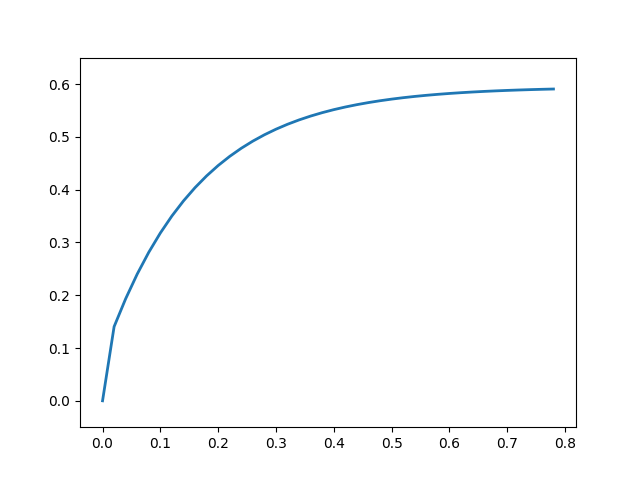
\includegraphics[width=100mm]{Figure_1.png}
    \end{center}
\end{figure}

The following is the python code:
\begin{code}

    \hfil

\begin{verbatim}
import matplotlib.pyplot as plt
import numpy as np
import math

#define constant
c = 2
P = 2
t_0 = 1/(2*c*math.sqrt(P))-1/(2*math.sqrt(c*math.sqrt(P)))+1/8 #switching time
C = (math.sqrt(2*t_0)-1/math.sqrt(c*math.sqrt(P)))
    *math.exp((c*math.sqrt(P)+2*math.sqrt(c*math.sqrt(P)))*t_0) 
    #constant for exponential function

#define velocity
def v(t):
 if(t <= t_0): return math.sqrt(2*t) #ignore air resistance
 else: return C*math.exp(-(c*math.sqrt(P)+2*math.sqrt(c*math.sqrt(P)))*t)
              +1/math.sqrt(c*math.sqrt(P)) #include air resistance, approximated

#plot velocity
t = np.arange(0, 0.8, 0.02)

velocity = []
for i in range(len(t)):
   velocity.append(v(t[i]))

plt.plot(t,velocity, lw=2)
plt.ylim(-0.05,0.65)

plt.show()
\end{verbatim}
\end{code}

\hfil

\subsection*{(e)}
Finally, using $\tilde{t}=\frac{t}{t_0}=\frac{t}{m}$, and $\tilde{v}=\frac{v}{v_0}=\frac{v}{\sqrt{P}}$ from part (a), plug back in to the function got in (d), it is as follow:
$$v(t)=\sqrt{P}\tilde{v}(t) = \begin{cases}
    \sqrt{\frac{2Pt}{m}} & t\leq m\tilde{t_*}\\
    C''''\exp\left(-\left(c\sqrt{P}+2\sqrt{c\sqrt{P}}\right)\frac{t}{m}\right)+\frac{1}{\sqrt{c\sqrt{P}}} & t> m\tilde{t_*}
\end{cases}$$ 
Where $C''''$ and $\tilde{t_*}$ are given in part (d).

Now, given that terminal velocity $v_t = \sqrt{P}\tilde{v_t} = \sqrt{P}\cdot \frac{1}{\sqrt{c\sqrt{P}}} = \sqrt{\frac{\sqrt{P}}{c}}$, if we want $v(t) = 0.99 v_t$ (99\% terminal velocity), it uses the second function, which we want the following:
$$C''''\exp\left(-\left(c\sqrt{P}+2\sqrt{c\sqrt{P}}\right)\frac{t}{m}\right)+\frac{1}{\sqrt{c\sqrt{P}}} = 0.99\frac{1}{\sqrt{c\sqrt{P}}}$$
$$\implies \exp\left(-\left(c\sqrt{P}+2\sqrt{c\sqrt{P}}\right)\frac{t}{m}\right) = -\frac{1}{100C''''\sqrt{c\sqrt{P}}}$$
$$\implies -\left(c\sqrt{P}+2\sqrt{c\sqrt{P}}\right)\frac{t}{m}=\ln\left(-\frac{1}{100C''''\sqrt{c\sqrt{P}}}\right)$$
$$\implies t=-\frac{m\ln\left(-\frac{1}{100C''''\sqrt{c\sqrt{P}}}\right)}{\left(c\sqrt{P}+2\sqrt{c\sqrt{P}}\right)}$$
Where $C'''' = \left(\sqrt{\frac{1}{c\sqrt{P}}-\frac{1}{\sqrt{c\sqrt{P}}}+\frac{1}{4}}-\frac{1}{\sqrt{c\sqrt{P}}}\right)\exp\left(\left(c\sqrt{P}+2\sqrt{c\sqrt{P}}\right)\left(\frac{1}{2c\sqrt{P}}-\frac{1}{2\sqrt{c\sqrt{P}}}+\frac{1}{8}\right)\right)$.
\end{comment}

\section{}%3
\begin{question}\label{q3}
    Consider an object, such as a car, with mass $m$, starting from rest, moving in one dimension, and subject to two forces. One, provided by an engine with a certain power output, is $F_e = P/v$. The other is some quadratic drag from air resistance, $F_d = -cv^2$.$P,c$ are both positive constants. Unfortunately, it is not possible to analytically solve for the car's velocity as a function of time. However, we can get approximate analytic expressions which are very accurate.
    \begin{itemize}
        \item[(a)] Calculate the terminal velocity $v_t$, and use it to define a dimensionless velocity variable $\tilde{v}=\frac{v}{v_t}$. Similarly, determine a timescale $\tau$ from the constant parameters in the problem, and use it to define a dimensionless time variable $\tilde{t}=\frac{t}{\tau}$. Write Newton's second law in terms of these dimensionless variables.
        \item[(b)] At the start of the motion, $\tilde{v}<< 1$, so air resistance is a small correction; the car's motion is essentially just acceleration driven by the engine. By ignoring the force due to air resistance, determine an (approximate) formula $\tilde{v}(\tilde{t})$, valid for $\tilde{v}<<1$.
        \item[(c)]Eventually, the car approaches terminal velocity. We can define 
        $$\epsilon = \tilde{v}_t-\tilde{v}$$
        If the car is going close to terminal velocity, $\epsilon <<1$. Expand the forces to linear order in $\epsilon$, and solve to get an (approximate) formula $\epsilon(\tilde{t})$, valid for $\epsilon<<1$.
        \item[(d)] Now comes the leap of faith: assume that either the velocity is small enough to ignore air resistance or the velocity is close to terminal velocity. In other words, we'll write $\tilde{v}(\tilde{t})$ as a piecewise function; before some time $\tilde{t}_*$ it takes the form of your solution to (c). Choose an appropriate switching time $\tilde{t}_*$ and write down such a piecewise function for $\tilde{v}(\tilde{t})$. You should fix the two undetermined constants by using that (i) the car starts at rest and (ii) $\tilde{v}$ should be continuous.Plot the piecewise function $\tilde{v}(\tilde{t})$.
        \item[(e)] Put all the constants back in to get $v(t)$. At what time $t$ does the car obtain $99\%$ of terminal velocity? You should give an analytic expression (using your approximate $\tilde{v}$). 
    \end{itemize}
\end{question}
\textbf{Pf:}

\subsection*{(a)}
First, assuming the mass of the object is not changing, then we get the differential equation $F = m\frac{dv}{dt} = F_e + F_d = \frac{P}{v}-cv^2$ (the total force given). From a physical interpretation, the object would reach terminal velocity, hence as $t\rightarrow\infty$, we get $\frac{dv}{dt}\rightarrow 0$, and $v\rightarrow v_t$. So, we get the following equation:
$$0 = \frac{P}{v_t}-cv_t^2 \implies cv_t^3 = P\implies v_t = \sqrt[3]{\frac{P}{c}}$$
Then, define $\tilde{v}=\frac{v}{v_t} = \sqrt[3]{\frac{c}{P}}v$ and $\tilde{t}=\frac{t}{\tau}$ (for some yet to be determined $\tau>0$), we get the following relationship:
$$\frac{d\tilde{v}}{d\tilde{t}} = \frac{d\tilde{v}}{dt}\cdot \frac{dt}{d\tilde{t}} = \frac{1}{v_t}\frac{dv}{dt}\cdot \tau = \frac{\tau}{v_t}\frac{dv}{dt}\implies \frac{dv}{dt}=\frac{v_t}{\tau}\frac{d\tilde{v}}{d\tilde{t}}$$
Plug back into the differential equation, we get:
$$\frac{mv_t}{\tau}\frac{d\tilde{v}}{d\tilde{t}}=\frac{P}{v_t\tilde{v}}-cv_t^2\tilde{v}^2\implies \frac{d\tilde{v}}{d\tilde{t}} = \frac{\tau P}{mv_t^2\tilde{v}}-\frac{c\tau v_t}{m}\tilde{v}^2$$
Define $\tau := \frac{mv_t^2}{P}$, we get the differential equation as follow:
$$\frac{d\tilde{v}}{d\tilde{t}} = \frac{1}{\tilde{v}}-\frac{cv_t^3}{P}\tilde{v}^2$$
Also, with $v_t =\sqrt[3]{\frac{P}{c}}$, $\frac{cv_t^3}{P}=1$, hence the differential equation becomes:
$$\frac{d\tilde{v}}{d\tilde{t}} = \frac{1}{\tilde{v}}-\tilde{v}^2$$

\subsection*{(b)}
If initially assume $\tilde{v}<<1$ (where air resistance is negligible), then we have $c=0$ (or the quadratic term is negligible). Hence, the differential equation in part (a) simplified to the following:
$$\frac{d\tilde{v}}{d\tilde{t}}=\frac{1}{\tilde{v}}\implies \tilde{v}\frac{d\tilde{v}}{d\tilde{t}}=1$$
Solving the differential equation, we get:
$$\int \tilde{v}\frac{d\tilde{v}}{d\tilde{t}}d\tilde{t} = \int 1d\tilde{t}\implies \frac{1}{2}\tilde{v}^2=\tilde{t}+C\implies \tilde{v} = \pm\sqrt{2\tilde{t}+C'}$$
Which, with the assumption that $t=0$ satisfies $v(0) = 0$ (initially at rest), we can derive $\tilde{t}=0$ satisfies $\tilde{v}(0) = 0$; also, WLOG, can assume the velocity is positive (can assume the engine powers the object in a way that the object moves in the positive direction). Hence, $C' = 0$, showing that $\tilde{v}(\tilde{t})=\sqrt{2\tilde{t}}$.

\subsection*{(c)}
When approaching terminal velocity (where $\epsilon = 1-\tilde{v}$ is small, with $\epsilon<<1$), we'll substitute $\tilde{v}$ with $\epsilon$. Where, we get the following:
$$\frac{d\epsilon}{d\tilde{t}}=-\frac{d\tilde{v}}{d\tilde{t}},\quad \tilde{v}=1-\epsilon$$
Hence, the differential equation can be expressed as:
$$-\frac{d\epsilon}{d\tilde{t}}=\frac{d\tilde{v}}{d\tilde{t}}= \frac{1}{\tilde{v}}-\tilde{v}^2 = \frac{1}{1-\epsilon}-(1-2\epsilon+\epsilon^2)$$
Which, since $\epsilon<1$, then the using the taylor series, $\frac{1}{1-\epsilon} =\sum_{k=0}^{\infty}\epsilon^k$. If we extract all the above terms up to linear order, we get the following approximation:
$$-\frac{d\epsilon}{d\tilde{t}}=(1+\epsilon)-(1-2\epsilon)\implies \frac{d\epsilon}{d\tilde{t}}=-3\epsilon \implies \epsilon = Ke^{-3\tilde{t}}$$
Here, $K$ depends on the initial condition provided. Which, by the definition of $\epsilon=1-\tilde{v}$, we get the following:
$$\tilde{v}=1-\epsilon = 1+K'e^{-3\tilde{t}}$$

\subsection*{(d)}
Given the information, we want the time $\tilde{t}\leq \tilde{t_*}$ to satisfy the equation in (b), while $\tilde{t}>\tilde{t_*}$ to satisfy the equation in (c), and the velocity is continuous (for some yet to be determined $\tilde{t_*}$). Which, we want a function in the following form:
$$\tilde{v}(\tilde{t})=\begin{cases}
    \sqrt{2\tilde{t}} & \tilde{t}\leq\tilde{t_*}\\
    1+K'e^{-3t} & \tilde{t}>\tilde{t_*}
\end{cases}$$
If we choose when $\tilde{v}=\frac{1}{2}$ to switch (i.e. when $\epsilon = 1-\tilde{v} = \frac{1}{2}<1$, up to half of the terminal velocity), we get the following for $\tilde{t_*}$:
$$\sqrt{2\tilde{t_*}} = \frac{1}{2}\implies \tilde{t_*}= \frac{1}{8}$$
And, for the function to be continuous, we want the right limit to be $\frac{1}{2}$ also (because the second function is continuous, this is the same as the evaluation of the second function that $\tilde{t_*}=\frac{1}{8}$). Then, we get the following:
$$1+K'e^{-3\cdot\frac{1}{8}} = \frac{1}{2}\implies K' = -\frac{1}{2}e^{\frac{3}{8}}$$
Then, the general form of the function becomes:
$$\tilde{v}(\tilde{t})=\begin{cases}
    \sqrt{2\tilde{t}} & \tilde{t}\leq \frac{1}{8}\\
    1-\frac{1}{2}e^{-3t+3/8} & \tilde{t}>\frac{1}{8}
\end{cases}$$
Using graphing program, the following is the graph (where the horizontal axis is $\tilde{t}$, vertical axis is $\tilde{v}$):
\begin{figure}[h!]
    \begin{center}
        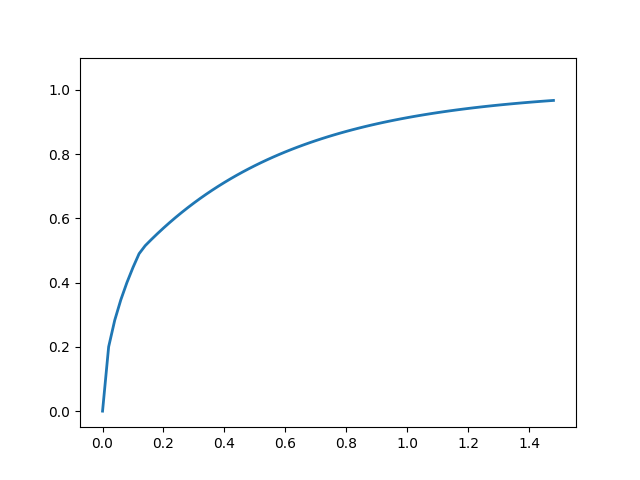
\includegraphics[width = 100mm]{Question 3 plot.png}
    \end{center}
\end{figure}

And, the following is the utilized code (programming language: python):

\rule{15.24cm}{0.01mm}
\begin{verbatim}
import matplotlib.pyplot as plt
import numpy as np
import math

#define constant
c = 2
P = 8
t_0 = 1/8
v_t = (P/c)**(1/3)

#define velocity
def v(t):
 if(t <= t_0): return math.sqrt(2*t) #ignore air resistance
 else: return 1-1/2*math.exp(-3*(t-1/8)) #include air resistance

#plot velocity
t = np.arange(0, 1.5, 0.02)

velocity = []
for i in range(len(t)):
   velocity.append(v(t[i]))

plt.plot(t,velocity, lw=2)
plt.ylim(-0.05,1.1)

plt.show()
\end{verbatim}

\rule{15.24cm}{0.01mm}

\subsection*{(e)}
If reconsider the relation $v = v_t\tilde{v}$, $\tilde{t}=\frac{t}{\tau}$, $v_t=\sqrt[3]{\frac{P}{c}}$, and $\tau = \frac{mv_t^2}{P}$. Plug these relations to the function in part (d), we get the following:
$$v(t) = \begin{cases}
    v_t\sqrt{\frac{2t}{\tau}} & t\leq \frac{1}{8}\tau\\
    v_t\left(1-\frac{1}{2}e^{-3\frac{t}{\tau}+3/8}\right) & t>\frac{1}{8}\tau
\end{cases}\quad = \begin{cases}
    \sqrt{\frac{2Pt}{m}} & t\leq \frac{m}{8\cdot P^{1/3}\cdot c^{2/3}}\\
    \sqrt[3]{\frac{P}{c}}-\frac{1}{2}\sqrt[3]{\frac{P}{c}}\exp\left(-\frac{3\cdot P^{1/3}\cdot c^{2/3}t}{m}+\frac{3}{8}\right) & t>\frac{m}{8\cdot P^{1/3}\cdot c^{2/3}}
\end{cases}$$
If the velocity approaches $0.99 v_t$ (99\% terminal velocity), it's equivalent to $\tilde{v}(\tilde{t}) = 0.99$, hence we get the followingtime variable:
$$\tilde{v}(\tilde{t})=1-\frac{1}{2}e^{-3\tilde{t}+3/8} = 0.99 \implies e^{-3\tilde{t}+3/8} = \frac{1}{50}\implies -3\tilde{t}+\frac{3}{8}=-\ln(50)$$
$$\implies \tilde{t} = \frac{1}{8}+\frac{\ln(50)}{3}$$
With $\tilde{t} = \frac{t}{\tau}$, we derive the following time:
$$t = \tau\left(\frac{1}{8}+\frac{\ln(50)}{3}\right) = \left(\frac{1}{8}+\frac{\ln(50)}{3}\right)\cdot \frac{m}{P^{1/3}\cdot c^{2/3}}$$

\break

\section{}%4
\begin{question}\label{q4}
    Consider a circular hoop (mass $M$ and radius $R$) standing vertically on the ground. Onto the hoop are threaded two beads (each mass $m$ and radius $r$), which move without friction along the hoop. The two beads start at rest practically at the top of the hoop (which requires $r<<R$; you can and should approximate for this being the case). One bead goes counterclockwise and the other clockwise.
    \begin{itemize}
        \item[(a)] What is the smallest value of $m/M$ for which the hoop rises off the ground?
        \item[(b)] Assuming the hoop does not rise off the ground, approximately how long does it take the beads to reach the bottom of the hoop? 
    \end{itemize}
\end{question}

\textbf{Pf:}

Since the beads appear on both sides, WLOG, can assume the behavior is symmetric, hence for the vertical components, we only need to analyze the bead on the right side.

\begin{figure}[h!]
    \begin{center}
        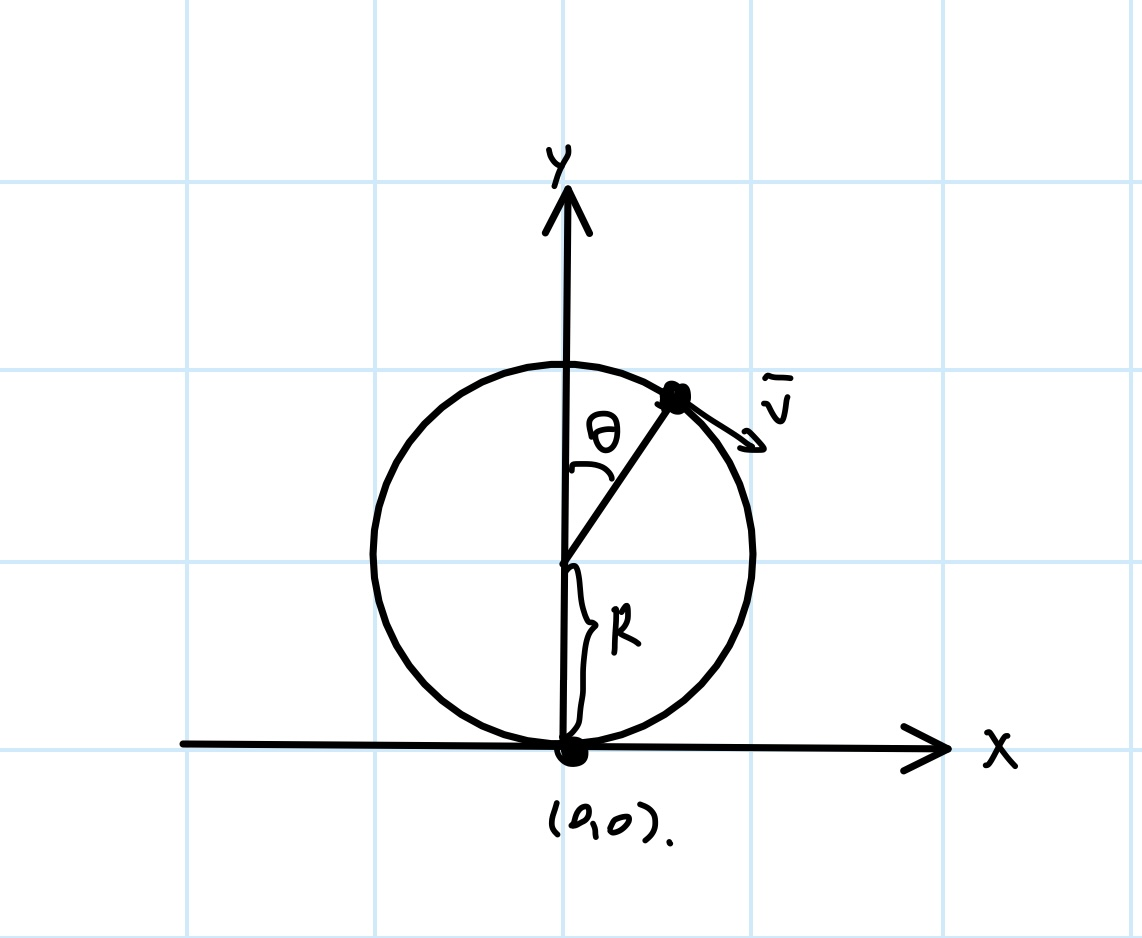
\includegraphics[width = 60mm]{q4 coord.jpg}
        \caption{The coordinates used in this question}
    \end{center}
\end{figure}

\subsection*{(a)}
First, for each angle $\theta$, the position of the bead is parametrized by:
$$\br(\theta)=(R\sin(\theta), R+R\cos(\theta))$$
Compared to the top (where height is $2R$), at angle $\theta$, the height drop is given by $2R-(R+R\cos(\theta)) = R(1-\cos(\theta))$, hence the lost potential energy of the bead is $mgR(1-\cos(\theta))$. If assume all the potential energy is transferred to kinetic energy, then $\frac{1}{2}mv^2 = mgR(1-\cos(\theta))$, hence at angle $\theta$, the speed of the bead satisfies:
$$v^2 = 2gR(1-\cos(\theta))\implies v=\sqrt{2gR(1-\cos(\theta))}$$
And, the unit tangent vector of the trajectory is given by:
$$\hat{v}(\theta)=\frac{\br'(\theta)}{|\br'(\theta)|} = \frac{1}{|\br'(\theta)|}(R\cos(\theta), -R\sin(\theta)) = (\cos(\theta),-\sin(\theta))$$

\hfil

Now, to calculate the acceleration on the bead, consider the following: Given some change in angle $\Delta\theta$, the distance this bead travels is about $\Delta x = R\Delta\theta$, and say the speed initially is given by $v$, then the change in time is approximately $\Delta t\approx\frac{\Delta x}{v} = \frac{R\Delta\theta}{v}$, hence $\frac{\Delta\theta}{\Delta t}\approx \frac{v}{R}$. Taking the limit, we get that $\frac{d\theta}{dt} = \frac{v}{R}$.

So, at each angle $\theta$, the velocity of the bead now is given by $\bv = v\hat{v} = \sqrt{2gR(1-\cos(\theta))}(\cos(\theta),-\sin(\theta))$. Then, the acceleration $\ba = \frac{d\bv}{dt} = \frac{d\bv}{d\theta}\cdot \frac{d\theta}{dt}$, which based on the formulas above, we get:
$$\frac{d\bv}{d\theta} = \frac{d}{d\theta}\left(\sqrt{2gR(1-\cos(\theta))}\right)\ (\cos(\theta),-\sin(\theta))+\sqrt{2gR(1-\cos(\theta))}\ \frac{d}{d\theta}\left((\cos(\theta),-\sin(\theta))\right)$$
$$ = \frac{2gR\sin(\theta)}{2\sqrt{2gR(1-\cos(\theta))}}(\cos(\theta),-\sin(\theta))+\sqrt{2gR(1-\cos(\theta))}(-\sin(\theta),-\cos(\theta))$$
$$ = \frac{gR\sin(\theta)}{v}(\cos(\theta),-\sin(\theta))-v(\sin(\theta),\cos(\theta))$$

$$\ba = \frac{d\bv}{d\theta}\cdot \frac{v}{R} = g\sin(\theta)(\cos(\theta),-\sin(\theta))-\frac{v^2}{R}(\sin(\theta),\cos(\theta))$$
$$ = g\sin(\theta)(\cos(\theta),-\sin(\theta))-2g(1-\cos(\theta))(\sin(\theta),\cos(\theta))$$
Hence, the vertical force component on the bead is given by:
$$\bF_y = m\ba_y = m\left(-g\sin^2(\theta)-2g(1-\cos(\theta))\cos(\theta)\right)\hat{y}$$
$$ = -mg((1-\cos^2(\theta))+(2\cos(\theta)-2\cos^2(\theta)))\hat{y}$$
$$= -mg(-3\cos^2(\theta)+2\cos(\theta)+1)\hat{y}$$
Let $\bF_b^{(y)}$ be the vertical force applied on the bead by the hoop, and $\bF_{g,h} = -mg\hat{y}$ be the gravity force applied on the bead. Then, for the bead to stay in the given motion with the proposed velocity, the net vertical force should be $\bF_y$. Hence, $\bF_b^{(y)}-mg\hat{y}=\bF_y$, or: 
$$\bF_b^{(y)}=\bF_y + mg\hat{y} = \left(mg-mg(-3\cos^2(\theta)+2\cos(\theta)+1)\right)\hat{y}$$
$$= mg(3\cos^2(\theta)-2\cos(\theta))\hat{y}$$
Let $\bF_h^{(y)}$ be the vertical force applied on the hoop by a single bead, using Newton's Third Law, $\bF_h^{(y)}=-\bF_b^{(y)}$, and since there are two beads, the vertical force applied on the hoop by the beads is:
$$2\bF_h^{(y)} = -2\bF_b^{(y)} = 2mg(2\cos(\theta)-3\cos^2(\theta))\hat{y} = mg(4\cos(\theta)-6\cos^2(\theta))\hat{y}$$

\hfil

Finally, for the hoop to rise off the ground, the vertical force applied on it should be directed upward. Since the only vertical forces are $2\bF_h^{(y)}$ and its gravity force $-Mg\hat{y}$, then the net vertical force is:
$$\bF_{y,\textmd{net}} = 2\bF_h^{(y)}-Mg\hat{y} = \left(mg(4\cos(\theta)-6\cos^2(\theta))-Mg\right)\hat{y}$$
For the force to be directed upward, the component is positive, hence this inequality is satisfied:
$$mg(4\cos(\theta)-6\cos^2(\theta))-Mg>0 \implies \frac{m}{M}(4\cos(\theta)-6\cos^2(\theta))>1$$ 
For $\cos(\theta)= \frac{1}{3}$, we have:
$$4\cos(\theta)-6\cos^2(\theta) =\frac{4}{3}-\frac{6}{9} = \frac{2}{3}>0$$
Hence, there are points where $4\cos(\theta)-6\cos^2(\theta)>0$ for $\theta\in [0,\pi]$ (the range of motion). Which, for $4\cos(\theta)-6\cos^2(\theta)>0$, the previous inequality can then be written as:
$$\frac{m}{M}>\frac{1}{4\cos(\theta)-6\cos^2(\theta)}$$
To find the infimum (intuitively, the smallest $\frac{m}{M}$ could approach), it suffices to find the maximum of $4\cos(\theta)-6\cos^2(\theta)$ for $\theta\in [0,\pi]$. Taking derivative being $0$, we get:
$$-4\sin(\theta)+12\cos(\theta)\sin(\theta)=0,\quad 4\sin(\theta)(3\cos(\theta)-1)=0$$
So, maximum happens at either $\sin(\theta)=0$ (which $\theta=0$ or $\pi$, including the boundary), or $\cos(\theta)=\frac{1}{3}$. Plug in the values, we get:
$$\theta=0\implies 4\cos(\theta)-6\cos^2(\theta) = 4-6=-2$$
$$\theta=\pi\implies 4\cos(\theta)-6\cos^2(\theta)=-4-6 = -10$$
$$\cos(\theta)=\frac{1}{3}\implies 4\cos(\theta)-6\cos^2(\theta) = \frac{4}{3}-\frac{6}{9} = \frac{2}{3}$$
Since $\frac{2}{3}$ is the largest, the maximum of $4\cos(\theta)-6\cos^2(\theta)$ on $[0,\pi]$ is $\frac{2}{3}$, hence the minimum of $\frac{1}{4\cos(\theta)-6\cos^2(\theta)} = \frac{3}{2}$ (for the denominator $>0$).

Hence, $\frac{m}{M}>\frac{3}{2}$ is the infimum ratio for the hoop to rise.
\subsection*{(b)}
Suppose the hoop doesn't rise, recall that for each $\Delta\theta$, the traveled distance for the bead is approximately $\Delta x\approx R\Delta\theta$, hence given speed $v$ at the initial point, the time elapsed during $\Delta x$ is $\Delta t\approx \frac{\Delta x}{v} \approx \frac{R}{v}\Delta \theta$, or $\frac{\Delta t}{\Delta\theta}\approx \frac{R}{v}$; thus taking the limit, $\frac{dt}{d\theta}=\frac{R}{v}$. 

\begin{figure}[h!]
    \begin{center}
        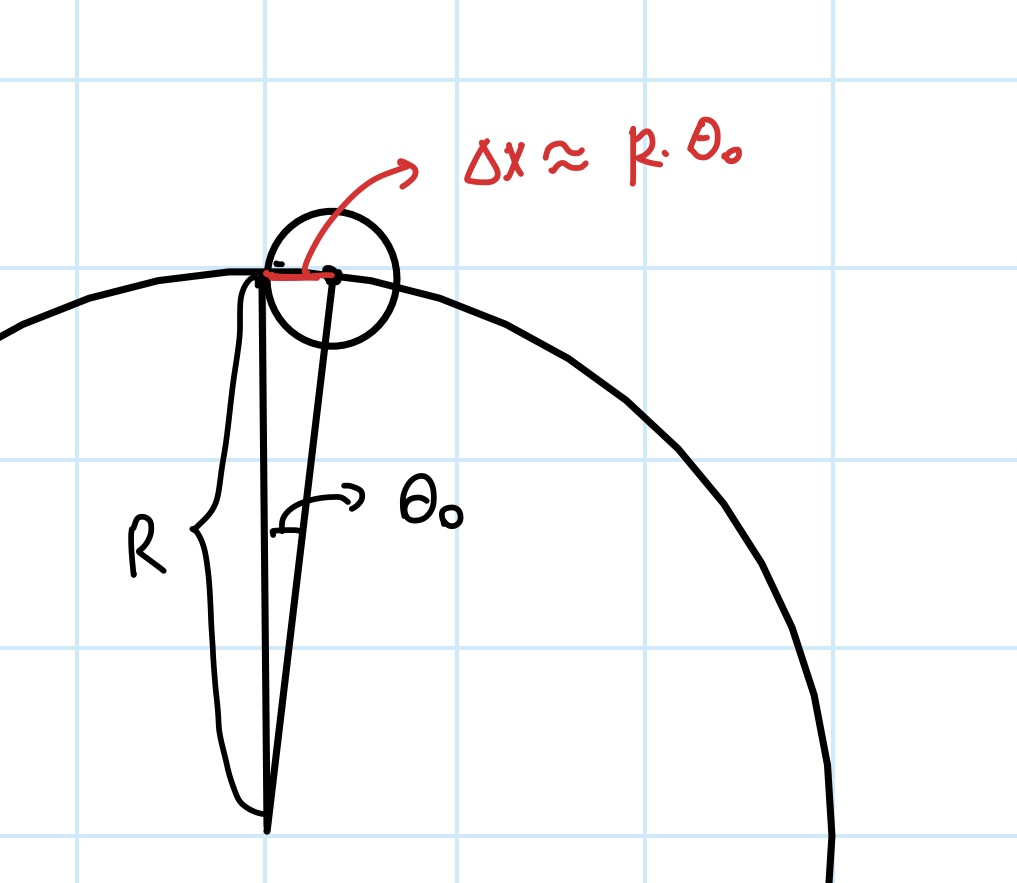
\includegraphics[width = 50mm]{q4 b.jpg}
        \caption{The bead's position near the top}
    \end{center}
\end{figure}

Now, notice that initially the beads are not directly on top (or $\theta_0>0$ initially), their centers are certain angle away from the top. Since $r<<R$, then we have $R\theta_0 \approx r$, hence $\theta_0 \approx \frac{r}{R}$ is the initial angle of the beads.

Also, When the beads fall to the ground, since $r<<R$, assume it approximately lands at $\theta_f=\pi$ (at the bottom). Then, with $v=\sqrt{2gR(1-\cos(\theta))}$, the time elapsed can be approximated as follow:
$$\Delta t \approx \int_{\theta_0}^{\theta_f}\frac{dt}{d\theta}d\theta = \int_{\frac{r}{R}}^{\pi}\frac{R}{\sqrt{2gR(1-\cos(\theta))}}d\theta = \sqrt{\frac{R}{g}}\int_{\frac{r}{R}}^{\pi}\frac{1}{\sqrt{2(1-\cos(\theta))}}d\theta$$
Now, given that $t=\frac{\theta}{2}$, we have the relation $2\sin^2(t) = 1-\cos(2t) = 1-\cos(\theta)$, and $dt = \frac{1}{2}d\theta$, then the above integral becomes:
$$\Delta t \approx 2\sqrt{\frac{R}{g}}\int_{\frac{r}{2R}}^{\frac{\pi}{2}}\frac{1}{\sqrt{2\cdot 2\sin^2(t)}}dt = 2\sqrt{\frac{R}{g}}\int_{\frac{r}{2R}}^{\frac{\pi}{2}}\frac{1}{2\sin(t)}dt = \sqrt{\frac{R}{g}}\int_{\frac{r}{2R}}^{\frac{\pi}{2}}csc(t)dt$$
$$ = -\sqrt{\frac{R}{g}}\ln(\cot(t)+\csc(t))\bigg|_{\frac{r}{2R}}^{\frac{\pi}{2}} = \sqrt{\frac{R}{g}}\ln\left(\cot\left(\frac{r}{2R}\right)+\csc\left(\frac{r}{2R}\right)\right)$$
Which, this is the approximated time the beads take to fall onto the ground.

\hfil

\hfil

\section{}%5
\begin{question}\label{q5}
    On the mastery questions, you showed that a rocket launched under the influence of gravity has a lower velocity, and that the "penalty" imposed by gravity is larger the longer it takes the rocket to burn its fuel. This suggests that, if launching to orbit off Earth, it would be best to make $dm/dt$ as large as possible. However, there's a technical challenge: burning fuel more rapidly generally requires a bigger engine, and the increasing mass of the engine imposes its own penalty. Let's take the rocket as having four components: fuel, fuel tank, engine, and payload initially, then 
    $$m_0 = m_f + m_t+m_e+m_p$$
    Let's assume that the rate of fuel consumption is proportional to the mass of the engine, 
    $$\alpha \equiv \left|\frac{dm}{dt}\right|=m_e/\tau$$
    and that the effective exhaust speed is fixed at $u$, regardless of the size of the engine. $\tau$ is some constant with units of time (it's the amount of time for the engine to consume a mass of fuel equal to its own mass), and for any particular rocket, $\alpha$ will be constnat.
    \begin{itemize}
        \item[(a)] Calculate the velocity of the racket after it has consumed all its fuel. Your answer should depend on $u,g,\tau$ and the masses of the four components.
        \item[(b)] Your final velocity should depend only on mass ratios, not the absolute masses. Explain physically why doubling the mass of everything has no effect on the final velocity.
        \item[(c)]Since only mass ratios are important, we can define $\tilde{m_i} = m_i/m_f$ (Remember that $f$ stands for fuel, not final). $\tilde{m_p}$ is fixed by a combination of the desired payload and how large a rocket we can build; $\tilde{m_t}$ is more or less fixed by choice of fuel. $\tilde{m_e}$ is the variable we have control over. Find the $\tilde{m_e}$ which maximizes the final speed as a function of $u,g,\tau,\tilde{m_p},\tilde{m_t}$.
        \item[(d)]For a chemical rocket, $u\sim 3 \textmd{km/s}$, $\tau\sim 7\textmd{s}$, and $\tilde{m_t}\sim 1/10$. Plug in numbers to get the optimal $\tilde{m_e}$ for both a negligible payload $(\tilde{m_p}=0$) and a modest payload ($\tilde{m_p}=0.1$). For both cases, also calculate the initial acceleration of the rocket, expressed as a number of $g$'s. 
    \end{itemize}
\end{question}

\textbf{Pf:}
\subsection*{(a)}
Recall the formula for the rate of change of time:
$$m\frac{dv}{dt}=u\frac{dm}{dt}+F_{\textmd{ext}}$$
Here, if we fix the upward direction as positive, then $F_{\textmd{ext}} = F_g = -mg$ (assume the only external force is the gravity, which is directed downward). Hence, with $m>0$ for all time $t$, the differential equation implies:
$$\frac{dv}{dt}=u\cdot\frac{1}{m}\frac{dm}{dt}-g$$

Also, since the mass is decreasing (always consuming fuel), we have $\frac{dm}{dt}=-\frac{m_e}{\tau}$ (which is constant), hence the time it takes to burn the fuel (with final mass $m_{\textmd{fin}} = m_t+m_e+m_p$), becomes:
$$\Delta t = \frac{m_{\textmd{fin}}-m_0}{dm/dt} = \frac{-m_f}{-m_e/\tau} = \frac{m_f\cdot \tau}{m_e}$$
Which, with the differential equation, the change in velocity becomes:
$$\Delta v=\int_0^{\Delta t}\frac{dv}{dt}dt = \int_0^{\frac{m_f\cdot \tau}{m_e}}\left(u\cdot\frac{1}{m}\frac{dm}{dt}-g\right)dt = u\ln(m(t))\bigg|_0^{\Delta t}-g\Delta t$$
$$=u\ln\left(\frac{m_{\textmd{fin}}}{m_0}\right)-\frac{g\cdot m_f\cdot \tau}{m_e} = u\ln\left(\frac{m_t+m_e+m_p}{m_f+m_t+m_e+m_p}\right)-\frac{g\cdot m_f\cdot \tau}{m_e}$$
(Note: $m(0) = m_0$, and $m(\Delta t)= m_\textmd{fin}$).

If assuming initiall $v_0=0$, then the above term provides the final velocity when the rocket consumes all its fuel.

\subsection*{(b)} 
Physically, when doubling the mass of everything, the gravity force applies on the rocket is larger at each moment, providing a larger negative acceleration than the original case; 

however, if $\tau$ (the time for the engine to consume the same mass of fuel as the engine's mass) doesn't change, then at any time period, the engine is also consuming a larger amount of fuel, causing $\frac{dm}{dt}$ to have a larger magnitude, and this provides a stronger thrusting force on the rocket. 

With both force components on the rocket increase (and point in different direction), their overall effect of the increase cancel out, leaving the rocket's change in velocity being affected only by the mass ratio.

\subsection*{(c)}
Recall that the velocity eventually is given as follow (with each index $i$, $\tilde{m_i} = \frac{m_i}{m_f}$):
$$v_\textmd{fin} = u\ln\left(\frac{m_t+m_e+m_p}{m_f+m_t+m_e+m_p}\right)-\frac{g\cdot m_f\cdot\tau}{m_e} = u\ln\left(\frac{\tilde{m_e}+\tilde{m_t}+\tilde{m_p}}{\tilde{m_e}+1+\tilde{m_t}+\tilde{m_p}}\right) - \frac{g\cdot \tau}{\tilde{m_e}}$$
Let $x=\tilde{m_e}$ for simplicity, final velocity as a function of $x$ is given by:
$$v_\textmd{fin}(x) = u\ln\left(\frac{x+\tilde{m_t}+\tilde{m_p}}{x+1+\tilde{m_t}+\tilde{m_p}}\right) - \frac{g\cdot\tau}{x}$$
$$ = u\ln(x+\tilde{m_t}+\tilde{m_p})-u\ln(x+1+\tilde{m_t}+\tilde{m_p})-\frac{g\tau}{x}$$
To find the maximum for $x>0$, taking the derivative and evaluate to be $0$, we get:
$$\frac{u}{x+\tilde{m_t}+\tilde{m_p}}-\frac{u}{x+1+\tilde{m_t}+\tilde{m_p}}+\frac{g\tau}{x^2} = 0$$
$$\implies \frac{u}{(x+\tilde{m_t}+\tilde{m_p})(x+1+\tilde{m_t}+\tilde{m_p})}=-\frac{g\tau}{x^2}$$
$$\implies ux^2 = -g\tau(x^2+(1+2\tilde{m_t}+2\tilde{m_p})x+(\tilde{m_t}+\tilde{m_p})(1+\tilde{m_t}+\tilde{m_p}))$$
$$\implies (u+g\tau)x^2+g\tau(1+2\tilde{m_t}+2\tilde{m_p})x+g\tau(\tilde{m_t}+\tilde{m_p})(1+\tilde{m_t}+\tilde{m_p})=0$$
Which, using quadratic formula, we get the following expression of $x$:
$$x=\tilde{m_e}=\frac{-g\tau(1+2\tilde{m_t}+2\tilde{m_p})\pm\sqrt{g^2\tau^2(1+2\tilde{m_t}+2\tilde{m_p})^2-4g\tau(u+g\tau)(\tilde{m_t}+\tilde{m_p})(1+\tilde{m_t}+\tilde{m_p})}}{2(u+g\tau)}$$
With the restriction that $x>0$, the $\pm$ will be dependent on the actual values, and the chosen units for each constants.

\subsection*{(d)}
Given that $u=3\textmd{km/s}$, $\tau = 7\textmd{s}$, and $\tilde{m_t}=\frac{1}{10}=0.1$. Since the speed is given in km/s, convert $g = 9.8 \textmd{m/s}^2 = 9.8\cdot 10^{-3}\textmd{km/s}^2$. Also, since $u$ represents the relative velocity of the fuel flow from the rocket, with the fuel propelled in the negative direction, $u=-3$ needs to be used.

Also, recall the acceleration formula is given by follow in part (a):
$$\frac{dv}{dt}=u\cdot\frac{1}{m}\frac{dm}{dt}-g$$
If we define $\tilde{m} = \frac{m}{m_f}$, we have $\tilde{m_0} = \frac{m_f+m_t+m_e+m_g}{m_f} = 1+\tilde{m_t}+\tilde{m_e}+\tilde{m_g}$, and $\frac{d\tilde{m}}{dt} = \frac{1}{m_f}\frac{dm}{dt}$, then the differential equation becomes:
$$\frac{dv}{dt}=u\cdot \frac{1}{\tilde{m}\cdot m_f}\cdot m_f\frac{d\tilde{m}}{dt}-g = u\cdot\frac{1}{\tilde{m}}\cdot\frac{d\tilde{m}}{dt}-g$$
And, as $\frac{dm}{dt} = -\frac{m_e}{\tau}$, $\frac{d\tilde{m}}{dt} = -\frac{1}{m_f}\cdot \frac{m_e}{\tau} = -\frac{\tilde{m_e}}{\tau}$.
\subsubsection*{1) When $\tilde{m_p}=0$:}
Plug into the formula for $\tilde{m_e}>0$ in part (c), we get:
$$\tilde{m_e} \approx 0.0667 $$
For the initial acceleration (with $\tilde{m} = \tilde{m_0}$), plug in the numbers, we get:
$$\frac{dv}{dt}\bigg|_{t=0} = (-3)\cdot\frac{1}{1+0.1+0.0667+0}\cdot\left(-\frac{0.0667}{7}\right)-g \approx 0.0245-g$$
(Note: $g=9.8\cdot 10^{-3}$ here is in km/s$^2$, based on the conversion of the units, the same applies to $\frac{dv}{dt}$).

\subsubsection*{2) When $\tilde{m_p}=0.1$:}
Plug into the formula again, we get:
$$\tilde{m_e} \approx 0.0931$$
Plug in all the numbers to get initial acceleration, we get:
$$\frac{dv}{dt}\bigg|_{t=0} = (-3)\cdot\frac{1}{1+0.1+0.0931+0.1}\cdot\left(-\frac{0.0931}{7}\right)-g \approx 0.0334-g$$
(Again, here $\frac{dv}{dt}$ is in km/s$^2$). 


\break

\section{Extra Credit}%6
\begin{question}\label{q6}
    Consider an object of mass $m$ moving in one dimension subject to three resistive forces: a constant frictional force with magnitude $\mu mg$, linear air resistance with magnitude $bv$, and quadratic air resistance with magnitude $cv^2$. If object starts with speed $v_0$, how long does it take to come to rest?
\end{question}

\textbf{Pf:}

Set the traveling direction to be positive, then the above resistive forces are all directed in a negative direction. Hence, the differential equation of the force is given as follow:
$$F = m\frac{dv}{dt} = - cv^2- bv-\mu mg  \implies \frac{1}{v^2+\frac{b}{c}v+\frac{\mu mg}{c}}\frac{dv}{dt}=-\frac{c}{m}$$
Using quadratic formula, if $v^2+\frac{b}{c}v+\frac{\mu mg}{c}=0$, $v$ is expressed as:
$$v=-\frac{b}{2c}\pm\sqrt{\left(\frac{b}{2c}\right)^2-\frac{\mu mg}{c}}$$
Which, let $\alpha=-\frac{b}{2c}$ and $\beta = \sqrt{(\frac{b}{2c})^2-\frac{\mu mg}{c}}$, using partial fraction, the rational term of $v$ can be expressed as:
$$v^2+\frac{b}{c}v+\frac{\mu mg}{c} = (v-(\alpha+\beta))(v-(\alpha-\beta))$$
$$\frac{1}{v^2+\frac{b}{c}v+\frac{\mu mg}{c}}=\frac{A}{v-(\alpha+\beta)}+\frac{B}{v-(\alpha-\beta)}$$\
Solving for the coefficients $A,B$, $A=-B$, and $B=-\frac{1}{2\beta}$, then the differential equation becomes:
$$\frac{1}{2\beta}\left(\frac{1}{v-(\alpha+\beta)}-\frac{1}{v-(\alpha-\beta)}\right)\frac{dv}{dt}=-\frac{c}{m}$$
Taking the integral, we get:
$$\frac{1}{2\beta}\int\left(\frac{1}{v-(\alpha+\beta)}-\frac{1}{v-(\alpha-\beta)}\right)\frac{dv}{dt}dt = \frac{1}{2\beta}\ln\left(\frac{v-(\alpha+\beta)}{v-(\alpha-\beta)}\right)= \int\left(-\frac{c}{m}\right)dt = -\frac{c}{m}t+K$$

$$\implies \ln\left(\frac{v-(\alpha+\beta)}{v-(\alpha-\beta)}\right) = -\frac{2c\beta}{m}t+K'$$
For $t=0$, since $v(0)=v_0$, we get the following relationship:
$$\ln\left(\frac{v_0-(\alpha+\beta)}{v_0-(\alpha-\beta)}\right)=K'$$
Which, for some time $t$, if $v=0$, we get the following equality:
$$\ln\left(\frac{-(\alpha+\beta)}{-(\alpha-\beta)}\right) = \ln\left(\frac{\alpha+\beta}{\alpha-\beta}\right) = -\frac{2c\beta}{m}t + \ln\left(\frac{v_0-(\alpha+\beta)}{v_0-(\alpha-\beta)}\right)$$
$$\implies \frac{2c\beta}{m}t = \ln\left(\frac{v_0-(\alpha+\beta)}{v_0-(\alpha-\beta)}\right)-\ln\left(\frac{\alpha+\beta}{\alpha-\beta}\right)=\ln\left(\frac{(v_0-(\alpha+\beta))(\alpha-\beta)}{(v_0-(\alpha-\beta))(\alpha+\beta)}\right)$$
$$\implies t=\frac{m}{2c\beta}\ln\left(\frac{(v_0-\alpha-\beta)(\alpha-\beta)}{(v_0-\alpha+\beta)(\alpha+\beta)}\right)$$
Finally, with $\alpha=-\frac{b}{2c}$, and $\beta=\sqrt{\left(\frac{b}{2c}\right)^2-\frac{\mu mg}{c}}$, we get the following expression for the time it takes to come to rest:
$$t = \frac{m}{2c\sqrt{\left(\frac{b}{2c}\right)^2-\frac{\mu mg}{c}}}\ln\left(\frac{\left(v_0+\frac{b}{2c}-\sqrt{\left(\frac{b}{2c}\right)^2-\frac{\mu mg}{c}}\right)\left(-\frac{b}{2c}-\sqrt{\left(\frac{b}{2c}\right)^2-\frac{\mu mg}{c}}\right)}{\left(v_0+\frac{b}{2c}+\sqrt{\left(\frac{b}{2c}\right)^2-\frac{\mu mg}{c}}\right)\left(-\frac{b}{2c}+\sqrt{\left(\frac{b}{2c}\right)^2-\frac{\mu mg}{c}}\right)}\right)$$
\begin{comment}
$$\implies \frac{v-(\alpha+\beta)}{v-(\alpha-\beta)} = 1-\frac{2\beta}{v-(\alpha-\beta)} = K''\exp\left(-\frac{2c\beta}{m}t\right)$$
$$\implies 1-K''\exp\left(-\frac{2c\beta}{m}t\right) = \frac{2\beta}{v-(\alpha-\beta)}\implies v-(\alpha-\beta)= \frac{2\beta}{1-K''\exp\left(-\frac{2c\beta}{m}t\right)}$$
$$\implies v= \frac{2\beta}{1-K''\exp\left(-\frac{2c\beta}{m}t\right)}+(\alpha-\beta)$$

Since for $t=0$, $v(0)=v_0$, then we get the following equality:
$$v_0 = \frac{2\beta}{1-K''}+(\alpha-\beta) \implies \frac{v_0-\alpha+\beta}{2\beta} = \frac{1}{1-K''}\implies 1-K'' = \frac{2\beta}{v_0-\alpha+\beta}\implies K'' = 1-\frac{2\beta}{v_0-\alpha+\beta}$$
Hence, the precise expression of velocity is:
$$v(t) = \frac{2\beta}{1-\left(1-\frac{2\beta}{v_0-\alpha+\beta}\right)\exp\left(-\frac{2c\beta}{m}t\right)}+(\alpha-\beta)$$

\hfil

To calculate when it stops, we need $v(t)=0$, hence, we get:
$$\frac{2\beta}{1-\left(1-\frac{2\beta}{v_0-\alpha+\beta}\right)\exp\left(-\frac{2c\beta}{m}t\right)}+(\alpha-\beta) = 0\implies \frac{2\beta}{\alpha-\beta}=\left(1-\frac{2\beta}{v_0-\alpha+\beta}\right)\exp\left(-\frac{2c\beta}{m}t\right)-1$$
$$\implies \exp\left(-\frac{2c\beta}{m}t\right) = \frac{\frac{2\beta}{\alpha-\beta}-1}{(1-\frac{2\beta}{v_0-\alpha+\beta})} = \frac{3\beta-\alpha}{\alpha-\beta}\cdot \frac{v_0-\alpha+\beta}{v_0-\alpha-\beta}$$
$$\implies -\frac{2c\beta}{m}t = \ln\left(\frac{3\beta-\alpha}{\alpha-\beta}\cdot \frac{v_0-\alpha+\beta}{v_0-\alpha-\beta}\right)\implies t=-\frac{m}{2c\beta}\ln\left(\frac{3\beta-\alpha}{\alpha-\beta}\cdot \frac{v_0-\alpha+\beta}{v_0-\alpha-\beta}\right)$$
Plug the original definition
\end{comment}

\end{document}